% Source page: original p. 335 (PDF p. 31)
% Figure number: Figure 14
% Uncertainty notes: none
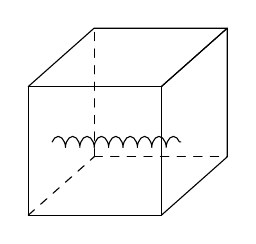
\begin{tikzpicture}[x=0.95cm,y=0.95cm,line cap=round,line join=round]
  \coordinate (A) at (0,0);
  \coordinate (B) at (1.78,0);
  \coordinate (C) at (1.78,1.72);
  \coordinate (D) at (0,1.72);
  \coordinate (E) at (0.88,0.78);
  \coordinate (F) at (2.66,0.78);
  \coordinate (G) at (2.66,2.50);
  \coordinate (H) at (0.88,2.50);

  \draw[dashed] (A) -- (E);
  \draw (A) -- (B) -- (C) -- (D) -- cycle;
  \draw (D) -- (H) -- (G) -- (C);
  \draw (C) -- (G);
  \draw (B) -- (F) -- (G);

  \draw[dashed] (E) -- (H);
  \draw[dashed] (E) -- (F);

  \draw[decorate,decoration={coil,aspect=0.45,segment length=5.2pt,amplitude=2.0pt}]
    (0.32,0.98) -- (2.04,0.98);
\end{tikzpicture}
